\section{Experiments}
\label{section:experiments}

In this section, we provide an empirical evaluation on our algorithms, verifying
their effectiveness on linearly separable datasets. We generated strongly and
weakly linearly separable datasets with $K=3$ classes in $\R^3$ i.i.d. from two
data distributions. Figures~\ref{figure:strongly-separable-dataset}
and~\ref{figure:weakly-separable-dataset} show visualizations of the two
datasets, along with detailed descriptions of the distributions.

\begin{figure}[h]
\centering
\begin{subfigure}[b]{0.23\textwidth}
\captionsetup{justification=centering}
\begin{center}
\hspace*{-0.3cm} 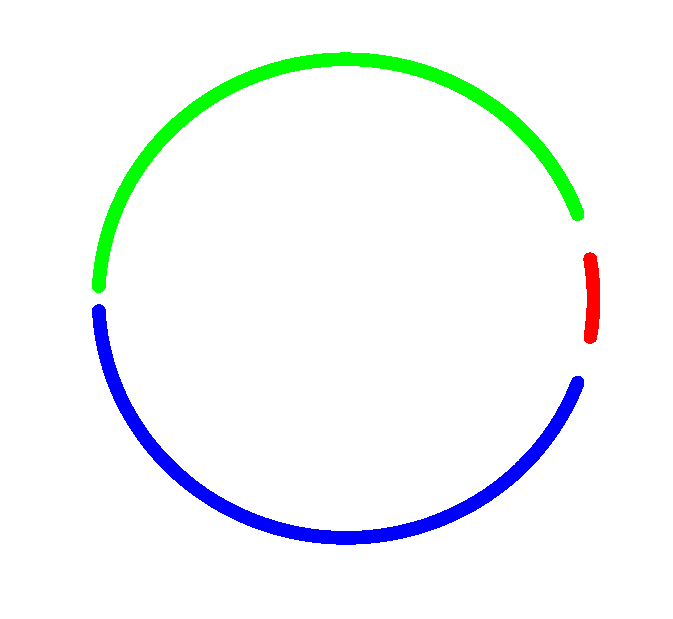
\includegraphics[width=1.15\textwidth, trim={0, 0cm, 0, 0}, clip]{figures/strong_points}
\caption{Strongly separable case}
\label{figure:strongly-separable-dataset}
\end{center}
\end{subfigure}
\hfill
\begin{subfigure}[b]{0.23\textwidth}
\captionsetup{justification=centering}
\centering
\hspace*{-0.3cm}  \includegraphics[width=1.15\textwidth, trim={0, 0cm, 0, 0}, clip]{figures/weak_points}
\caption{Weakly separable case}
\label{figure:weakly-separable-dataset}
\end{subfigure}
\vspace*{-0.2cm}
\caption{Strongly and weakly linearly separable datasets in $\R^3$ with $K=3$
classes and $T=5\times 10^6$ examples. Here we show projections of the examples
onto their first two coordinates, which lie in the ball of radius $1/\sqrt{2}$
centered at the origin. The third coordinate is $1/\sqrt{2}$ for all examples.
Class 1 is depicted red. Classes 2 and 3 are depicted green and blue,
respectively. $80\%$ of the examples belong to class 1, $10\%$ belong to class 2
and $10\%$ belong to class 3. Class 1 lies in the angle interval $[-15^\circ,
15^\circ]$, while classes 2 and 3 lie in the angle intervals $[15^\circ,
180^\circ]$ and $[-180^\circ, -15^\circ]$ respectively. The examples are
strongly and weakly linearly separable with a margin of $\gamma=0.05$,
respectively. (Examples lying within margin $\gamma$ of the linear separators
were rejected during sampling.)}
\label{figure:strongly-and-weakly-separable-datasets}
\end{figure}

We implemented
Algorithm~\ref{algorithm:algorithm-for-strongly-linearly-separable-examples},
Algorithm~\ref{algorithm:kernelized} with rational
kernel~\eqref{equation:rational-kernel}, and the \textsc{Banditron} algorithm.
We evaluated these algorithms on the two datasets. \textsc{Banditron} has an
exploration rate parameter, for which we tried values $0.02, 0.01, 0.005, 0.002,
0.001, 0.0005$. Since all three algorithms are randomized, we run each algorithm
$20$ times. The average cumulative number of mistakes up to round $t$ as a
function of $t$ are shown in
Figures~\ref{figure:number-of-mistakes-strongly-separable-dataset}
and~\ref{figure:number-of-mistakes-weakly-separable-dataset}.

We can see that there is a tradeoff in the setting of the exploration rate for
\textsc{Banditron}. With large exploration parameter, \textsc{Banditron} suffers
from over-exploration, whereas with small exploration parameter, its model
cannot be updated quickly enough. As expected,
Algorithm~\ref{algorithm:algorithm-for-strongly-linearly-separable-examples} has
a small number of mistakes in the strongly linearly separable setting, while
having a large number of mistakes in the weakly linearly separable setting, due
to the limited representation power of linear classifiers. In contrast,
Algorithm~\ref{algorithm:kernelized} with rational kernel has a small number of
mistakes in both settings, exhibiting strong adaptivity guarantees.
Appendix~\ref{section:supp-to-experiment} shows the decision boundaries that
each of the algorithms learns.

\begin{figure}
\centering
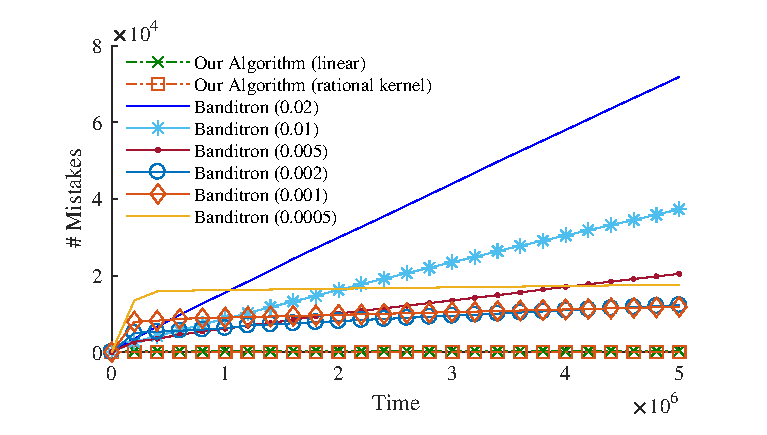
\includegraphics[width=0.42\textwidth]{figures/strong3}
\caption{Average cumulative number of mistakes of various algorithms versus the
number of rounds for the strongly linearly separable dataset of
\autoref{figure:strongly-separable-dataset}.}
\label{figure:number-of-mistakes-strongly-separable-dataset}
\end{figure}

\begin{figure}
\centering
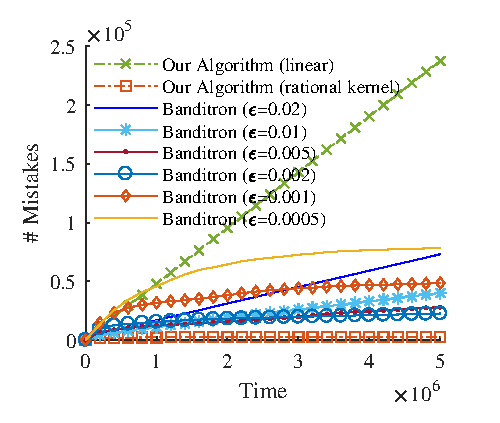
\includegraphics[width=0.42\textwidth]{figures/weak3}
\caption{Average cumulative number of mistakes of various algorithms versus the
number of rounds for the weakly linearly separable dataset of
\autoref{figure:weakly-separable-dataset}.}
\label{figure:number-of-mistakes-weakly-separable-dataset}
\end{figure}
